% Created 2016-05-23 ma. 16:26
\documentclass[11pt]{article}
\usepackage[utf8]{inputenc}
\usepackage[T1]{fontenc}
\usepackage{fixltx2e}
\usepackage{graphicx}
\usepackage{longtable}
\usepackage{float}
\usepackage{wrapfig}
\usepackage{rotating}
\usepackage[normalem]{ulem}
\usepackage{amsmath}
\usepackage{textcomp}
\usepackage{marvosym}
\usepackage{wasysym}
\usepackage{amssymb}
\usepackage{capt-of}
\usepackage{hyperref}
\tolerance=1000
\usepackage{minted}
\usepackage{tikz}
\usepackage{parskip}
\usepackage{color}
\usepackage{listings}
\usepackage{grffile}
\definecolor{mintedbackground}{rgb}{0.95,0.95,0.95}
\usepackage[inline]{enumitem}
\usepackage{tikz,graphicx, graphics, pgfkeys}
\usetikzlibrary{arrows,decorations.pathreplacing}
\usepackage{xcolor}
\hypersetup{
colorlinks,
linkcolor={red!50!black},
citecolor={blue!50!black},
urlcolor={blue!80!black}
}
\usepackage{setspace}%% The linestretch
\singlespacing
\usepackage[format=hang,indention=0cm,singlelinecheck=true,justification=raggedright,labelfont={normalsize,bf},textfont={normalsize}]{caption} %
\usepackage{vmargin}
\setpapersize{A4}
\setmarginsrb{2.5cm}{1cm}% links, oben
{2.5cm}{2cm}% rechts, unten
{12pt}{30pt}% Kopf: Höhe, Abstand
{12pt}{30pt}% Fuß: Höhe, AB
\usepackage{upquote}
%  use straight quotes when printing a command in minted
\AtBeginDocument{%
\def\PYZsq{\textquotesingle}%
}
\setlength{\parindent}{0pt}
\setlength{\parskip}{\baselineskip}
\definecolor{mintedbackground}{rgb}{0.95,0.95,0.95}
\author{Alexander Jueterbock, Martin Jakt\thanks{Nord University, Norway}}
\date{\textbf{PhD course: High throughput sequencing of non-model organisms}}
\title{\textbf{Trimming and quality control} (June 2016)}
\hypersetup{
 pdfkeywords={},
  pdfsubject={},
  pdfcreator={Emacs 24.5.1 (Org mode 8.3beta)}}
\begin{document}

\maketitle
\tableofcontents







After a general introduction to the UNIX command line, it is time for
you to analyze your own fastq files. The first important step for any
kind of sequencing data is to get rid of adapter contamination and 
bad quality reads. In this tutorial we will use the programs \href{http://www.bioinformatics.babraham.ac.uk/projects/fastqc/}{FastQC}
and \href{http://www.bioinformatics.babraham.ac.uk/projects/trim_galore/}{TrimGalore!} to check the quality of the sequenced libraries before
and after trimming.


\textbf{IMPORTANT NOTE} Before you get started: to compare characteristics of
your libraries, please keep record of the resulting numbers, like the
number of raw reads, reads after quality control, number of mapped
reads etc. This helps to identify peculiarities/outliers in your
libraries which may either be due to biological peculiarities of your
species or unknown technical issues.


Log on (with \texttt{ssh}) to the remote computer with the \texttt{-X} option (like
\texttt{ssh -x user@158...}) to be able to use graphical interfaces.

\section{Overview of sequence lengths}
\label{sec-1}
Next Generation Sequencing data is generally stored in fastq
files. Most of the time the data are compressed, either in .zip or in
.gz format.

If your file is zip-compressed, you can use the following command to unzip it:

\begin{minted}[fontsize=\scriptsize,bgcolor=lightgray,linenos]{sh}
unzip FILE.fastq.zip
\end{minted}

If your file iz gz-compressed, use the following command instead:

\begin{minted}[fontsize=\scriptsize,bgcolor=lightgray,linenos]{sh}
gunzip FILE.fastq.gz
\end{minted}

\textbf{NOTE}: For paired-end sequencing from Illumina, you have two
files. One file with the forward reads (\texttt{Sequence\_R1.fq}) and one file with
the reverse reads (\texttt{Sequence\_R2.fq}).


To get a quick impression of the minimum and maximum read lengths in
your fastq file, you can use the following commands (replace
\texttt{FILE.fastq} with your own filename):

\begin{minted}[fontsize=\scriptsize,bgcolor=lightgray,linenos]{sh}
awk '{if(NR%4==2) print length($0)}' FILE.fastq| sort -n | head -n1
awk '{if(NR%4==2) print length($0)}' FILE.fastq| sort -n | tail -n1
\end{minted}

It reads like this: measure the length of every second line in every
group of 4 lines (the sequence line in a fastq file), \texttt{sort} it
(numerically with \texttt{-n}) and print out either the first (smallest)
value with \texttt{head} or the last (biggest) value with \texttt{tail}. \texttt{NR}
represents the current line number and the \texttt{\%} sign is the modulus
operator, which divides the line number by 4 (\texttt{NR\%4}) and returns only
the remainder. This extracts all the sequences, which are on line
2,6,10,14\ldots{}


The following command allows you to count the sequence lengths:

\begin{minted}[fontsize=\scriptsize,bgcolor=lightgray,linenos]{sh}
awk '{if(NR%4==2) print length($0)}' FILE.fastq | sort -n | uniq -c > read_length.txt
\end{minted}

The lines that follow make use of the program R. If you copy and
paste the code into the command line, you will get an overview graphic
of the sequence length distribution 

\begin{minted}[fontsize=\scriptsize,bgcolor=lightgray,linenos]{sh}
cat >> Rplot.r << 'EOF'
reads<-read.csv(file="read_length.txt", sep="", header=FALSE)

png(filename = "SequenceLengthDistribution.png",
         width = 480, height = 480, units = "px", pointsize = 12,
          bg = "white")
plot(reads$V2,reads$V1,type="l",xlab="read length",ylab="occurences",col="blue")
dev.off()

EOF


R CMD BATCH Rplot.r
\end{minted}

You can open the created figure with the GNOME image viewer using the
following command:

\begin{minted}[fontsize=\scriptsize,bgcolor=lightgray,linenos]{sh}
eog SequenceLengthDistribution.png
\end{minted}


\begin{figure}[htb]
\centering
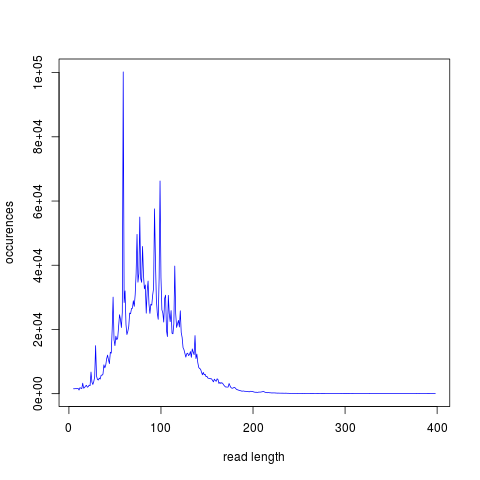
\includegraphics[width=10cm]{SequenceLengthDistribution.png}
\caption{Example graphic of the length distribution in a fastq file}
\end{figure}

Does the sequence length-distribution meet your expectations? 

\textbf{NOTE}: While the Ion Torrent sequences will differ in length (as in
Figure 1), the Illumina sequences will all have the same read length
(301 bp). 


\section{Quality control}
\label{sec-2}
To inspect the quality of the sequencing data, we use
\href{http://www.bioinformatics.babraham.ac.uk/projects/fastqc/}{FastQC}. In
the installation and setup instructions of the program
(\href{http://www.bioinformatics.babraham.ac.uk/projects/fastqc/INSTALL.txt}{link}),
you will find that FastQC can run in an interactive mode or in a
command line mode. This tutorial uses the command-line version.

FastQC knows a number of standard adapter sequences used for HTS,
including adapters used on Illumina platforms; To get an overview of
the contaminants (overrepresented sequences) that FastQC will look
for by default, type

\begin{minted}[fontsize=\scriptsize,bgcolor=lightgray,linenos]{sh}
less /usr/share/fastqc/Contaminants/contaminant_list.txt
\end{minted}

However, FastQC is not aware of the sequences used by the IonTorrent
platform. To inform FastQC of the Ion Torrent adapter sequences
call FastQC with the \texttt{-{}-contaminants} option to specify a file
containing the adapter sequences we have used.

So, to run FastQC on your file, type:

\begin{minted}[fontsize=\scriptsize,bgcolor=lightgray,linenos]{sh}
fastqc --contaminants adapters.txt FILE.fastq
\end{minted}

The adapters.txt file contains the adapter sequences in a
name[tab]sequence format, like

\begin{minted}[fontsize=\scriptsize,bgcolor=lightgray,linenos]{sh}
IonTorrentAAdapter      CCATCTCATCCCTGCGTGTCTCCGACTCAG
IontTorrentP1Adapter    CCACTACGCCTCCGCTTTCCTCTCTATGGGCAGTCGGTGAT
\end{minted}

You can create this file on the adapters.txt file on the remote computer with:

\begin{minted}[fontsize=\scriptsize,bgcolor=lightgray,linenos]{sh}
touch adapters.txt
\end{minted}

Open the text file with the program nano:

\begin{minted}[fontsize=\scriptsize,bgcolor=lightgray,linenos]{sh}
nano adapters.txt
\end{minted}

Then copy and paste the name-sequence combinations of the Ion Torrent
adapters (see above) into the file and close the file by pressing
Ctrl+O, then Ctrl+X on your keyboard.

The output of the FastQC program will be saved in a folder that has
the name of your fastq file and ends with fastqc, like
\texttt{FILE\_fastqc}. Use the \texttt{cd} command to move into the folder and open
the produced \texttt{fastqc\_report.html} either with \texttt{firefox} or
\texttt{chromium-browser} (one of the two should work).

\begin{minted}[fontsize=\scriptsize,bgcolor=lightgray,linenos]{sh}
cd FILE_fastqc
firefox fastqc_report.html
chromium-browser fastqc_report.html
\end{minted}

Scrolling through this html file on the remote computer will be quite
slow. it may be more convenient to copy the output folder to your
computer with \href{https://filezilla-project.org/}{FileZilla} or 'rsync' (see in the 'Unix tools' session) .
Get familiar with the output of each module.


For example, it is normal that the the per base sequence quality drops
towards the end of the read, as seen in Figure 2. In the next section
we will see how to trim away these low-quality reads.

\begin{figure}[htb]
\centering
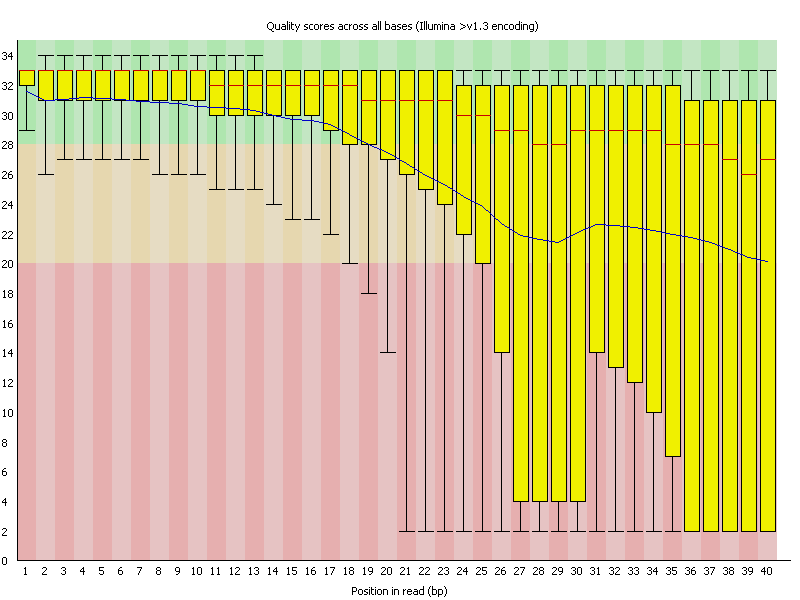
\includegraphics[width=10cm]{per_base_quality.png}
\caption{Per base sequence quality (from \href{http://www.bioinformatics.babraham.ac.uk/projects/fastqc/Help/3\%20Analysis\%20Modules/2\%20Per\%20Base\%20Sequence\%20Quality.html}{link})}
\end{figure}

The figure on duplication levels (Figure 3) informs you about the
percentage of duplicate reads in your sequenced library.  Duplicates
result from primer or PCR bias towards these reads.  As they can skew
genotype estimates, we will remove duplicate reads later in the week
before SNP calling.

\begin{figure}[htb]
\centering
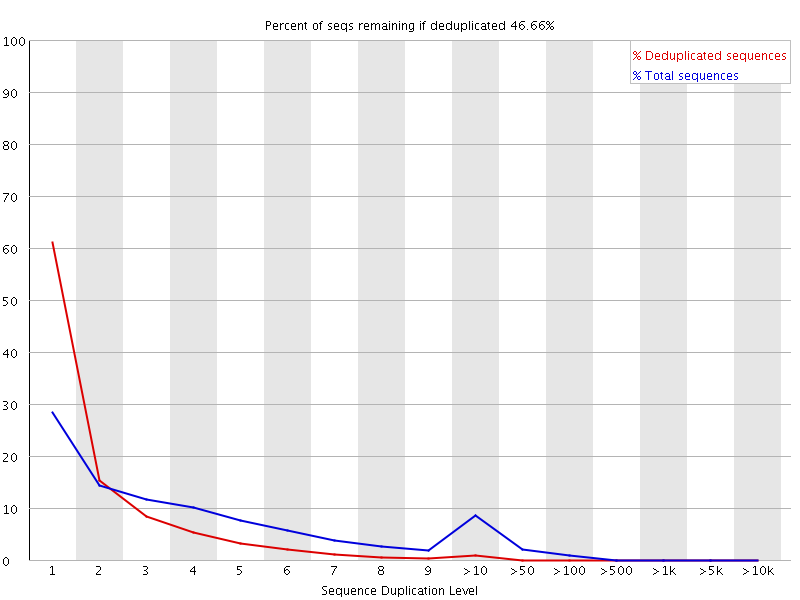
\includegraphics[width=10cm]{duplication_levels.png}
\caption{Per base sequence quality (from \href{http://www.bioinformatics.babraham.ac.uk/projects/fastqc/Help/3\%20Analysis\%20Modules/8\%20Duplicate\%20Sequences.html}{link})}
\end{figure}

You can find guidance on how to interpret the output of each module
\href{http://www.bioinformatics.babraham.ac.uk/projects/fastqc/Help/3\%20Analysis\%20Modules/}{here} 

\section{Trimming low quality reads and adapters}
\label{sec-3}
\href{http://www.bioinformatics.babraham.ac.uk/projects/trim_galore/}{TrimGalore!} is a wrapper script to automate quality and adapter
trimming as well as quality control (\href{http://www.bioinformatics.babraham.ac.uk/projects/trim_galore/trim_galore_User_Guide_v0.3.7.pdf}{User Guide}).

When the program is installed, it can be used with 

\begin{minted}[fontsize=\scriptsize,bgcolor=lightgray,linenos]{sh}
trim_galore [options] <filename(s)>
\end{minted}

You can get an overview of the options with the \texttt{-{}-help} option:

\begin{minted}[fontsize=\scriptsize,bgcolor=lightgray,linenos]{sh}
trim_galore --help
\end{minted}

With the default settings, TrimGalore! trims low-quality ends with a
Phred quality score threshold of 20 (can be changed with \texttt{-q}) and
discards reads that become shorter than 20 bp (can be changed with
\texttt{-{}-length}).

TrimGalore! uses the program \href{https://code.google.com/p/cutadapt/}{Cutadapt} to find and remove adapters from
the 3' end of the reads (see Fig. \ref{fig:adapters}). The program Cutadapt
itself gives you more options for adapter trimming and allows you to
remove adapters also from the 5'-end of the sequence (see
\url{http://cutadapt.readthedocs.org/en/latest/guide.html})

\begin{figure}[htb]
\centering
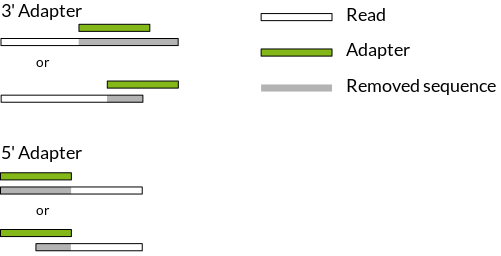
\includegraphics[width=14cm]{adapters.png}
\caption{\label{fig:adapters}3'- and 5'-adapter trimming (\href{http://cutadapt.readthedocs.org/en/latest/guide.html}{source})}
\end{figure}

\subsection{Trimming Ion-Torrent adapters}
\label{sec-3-1}

The Ion-P1- and Ion-A-adapters are supposed to be automatically
trimmed off on the Ion Server. So, the fastq files with the raw reads
should not contain these adapters anymore. Still, it is good to check
if there are any adapters left in your library - they can have
negative effects on further analyses.



The adapters used for Ion Torrent sequencing are shown in
Fig. \ref{fig:ionadapters} and their orientation in the libraries is shown
in Fig. \ref{fig:adapterorientations}.

\begin{figure}[htb]
\centering
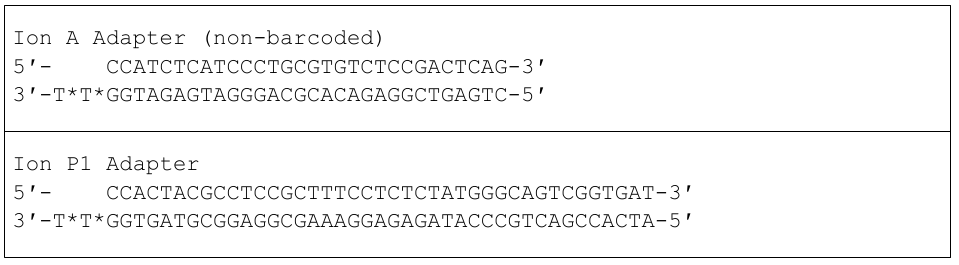
\includegraphics[width=14cm]{IonAdapters.png}
\caption{\label{fig:ionadapters}Non-barcoded Ion-A and -P1 adapter sequences. In each sequence, a "*" indicates a phosphorothioate bond, for protection from nucleases and to preserve the directionality of adapter ligation. This is not relevant for adapter trimming.}
\end{figure}

\begin{figure}[htb]
\centering
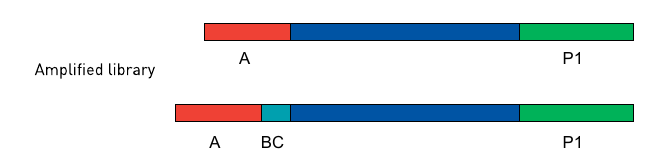
\includegraphics[width=14cm]{IonLibraryWithAdapters.png}
\caption{\label{fig:adapterorientations}Ion adapters in the amplified library. BC is an optional barcode sequence.}
\end{figure}.

To trim off the A-adapter, use TrimGalore! with the command:

\begin{minted}[fontsize=\scriptsize,bgcolor=lightgray,linenos]{sh}
trim_galore \
-a CCATCTCATCCCTGCGTGTCTCCGACTCAG \
--stringency 3 \
FILE.fastq
\end{minted}


The \texttt{\textbackslash{}} sign just means that the command continues on the next
line. You could type the entire command on a single line.


The option \texttt{-{}-stringency 3} means that a >3bp overlap with the adapter
sequence will be trimmed off the 3' end. The program writes a file
that ends with \texttt{trimming\_report.txt}, which reports the number of
reads that have been trimmed and/or removed.

The output file has the ending \texttt{trimmed.fq}. Use this file as
input to TrimGalore! to trim off the P1-adapter:

\begin{minted}[fontsize=\scriptsize,bgcolor=lightgray,linenos]{sh}
trim_galore \
-a CCACTACGCCTCCGCTTTCCTCTCTATGGGCAGTCGGTGAT \
--stringency 3 \
--fastqc FILE_trimmed.fq
\end{minted}

The \texttt{-{}-fastqc} option will automatically run FastQC in the default
mode. Compare the FastQC outputs before and after trimming.


\clearpage

\subsection{Trimming Illumina adapters}
\label{sec-3-2}
Depending on the settings for Illumina sequencing, the adapters can be
automatically removed from the fastq files that you get from the
sequencing machine. This, however, has to be defined before
sequencing. If you are not sure whether adapters have been trimmed off
or not, it is safe to trim the adapters before using the sequences for
any further analyses.

The Illumina adapters are as follows:

\begin{minted}[fontsize=\scriptsize,bgcolor=lightgray,linenos]{sh}
TruSeq Universal Adapter:
5' AATGATACGGCGACCACCGAGATCTACACTCTTTCCCTACACGACGCTCTTCCGATCT 3'

TruSeq Indexed Adapter
5' P*GATCGGAAGAGCACACGTCTGAACTCCAGTCACNNNNNNATCTCGTATGCCGTCTTCTGCTTG 3'
\end{minted}

Here, \texttt{NNNNNN} represents a barcode of six nucleotides in the indexed adapter.

TrimGalore! can be run with the option \texttt{-{}-illumina}. This trims the
first 13bp of the Illumina universal adapter \texttt{AGATCGGAAGAGC}. This
option removes illumina adapters from most standard libraries,
including TruSeq adapters.

The location of this sequence in the TruSeq adapter is shown here:

\begin{minted}[fontsize=\scriptsize,bgcolor=lightgray,linenos]{sh}
TruSeq Universal Adapter:
5' AATGATACGGCGACCACCGAGATCTACACTCTTTCCCTACACGACGCTCTTCCGATCT 3'
   Reverse                                      CGAGAAGGCTAGA 

TruSeq Indexed Adapter
5' P*GATCGGAAGAGCACACGTCTGAACTCCAGTCACNNNNNNATCTCGTATGCCGTCTTCTGCTTG 3'
    AGATCGGAAGAGC
\end{minted}

The A on the 5'-end of the TruSeq indexed adapter is added during
A-tailing of your DNA library fragments.
The orientation of the adapters in the illumina library are shown in Fig. \ref{fig:illuminaadapters}.
\begin{figure}[htb]
\centering
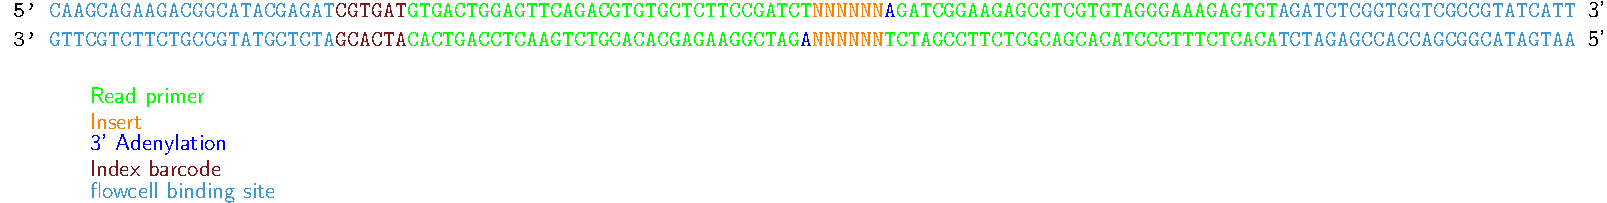
\includegraphics[width=17cm]{IlluminaAdaptersVisualized.pdf}
\caption{\label{fig:illuminaadapters}Orientation of the illumina adapters around the DNA inserts}
\end{figure}


TrimGalore! also performs trimming of paired-end libraries, as the
Illumina libraries that were prepared in this course. This allows to
discard too short read pairs without disturbing the sequence order of
FastQ files, which is required by many aligners.  With the option
\texttt{-{}-paired} TrimGalore! expects two paired fastq input files, like
\texttt{file1\_1.fq} and \texttt{file1\_2.fq}.  Here, both sequences of a sequence
pair must have a certain minimum length (specified by the \texttt{-{}-length}
option) in order to be kept. If only one of the two paired end reads
becomes too short, the option \texttt{-{}-retain\_unpaired} can be applied to
write the long-enough unpaired read to either \texttt{unpaired\_1.fq} or
\texttt{unpaired\_2.fq}. The length cutoff for unpaired single end reads is
governed by the parameters \texttt{-{}-length\_1} and \texttt{-{}-length\_2}

To trim our illumina paired-end libraries we can use:

\begin{minted}[fontsize=\scriptsize,bgcolor=lightgray,linenos]{sh}
trim_galore \
--illumina \
--stringency 3 \
--paired \
--retain_unpaired \
--length_1 21 \
--length_2 21 \
--fastqc \
Illumina_R1.fastq \
Illumina_R2.fastq
\end{minted}

This command runs automatically FastQC on the trimmed
libraries. Besides the \texttt{fastqc.html} files, you will find fastq files
with the validated sequences (\texttt{Illumina\_R1\_val\_1.fq},
\texttt{Illumina\_R2\_val\_2.fq}) and with the unpaired sequences
(\texttt{Illumina\_R1\_unpaired\_1.fq},=Illumina\(_{\text{R2}}_{\text{unpaired}}_{\text{2.fq}}\)=).  The files
ending with \texttt{trimming\_report.txt} provide information on the number of
reads that have been trimmed and/or removed.

You can now compare the quality of your raw libraries and your
quality-trimmed libraries. What did improve? Are there still any
problems with your libraries after trimming?
Emacs 24.5.1 (Org mode 8.3beta)
\end{document}